\section{\uppercase{Results}}
\label{sec:results}
\subsection{Exact Artifact Recovery and Useful Rate}
The prospective allocation completed all 120 stego outcomes and 40 independent controls. There were 100 exact, authenticated and conforming recoveries and 20 retained A1 text capacity failures. All 280 model processes have GPU execution evidence. No source replacement, protocol retry, timeout or infrastructure failure was needed. Table~\ref{tab:outcomes} and Figure~\ref{fig:recovery} retain every attempt.\aifootnote

\begin{table*}[t]
\caption{Prospective outcomes and original reference-path runtime. Each cell has 20 attempted payload groups. Exact recovery is 20/20 with 95\% interval [83.16\%, 100\%], or 0/20 with [0\%, 16.84\%]. Phase means exclude loading and some process overhead. Charged means include both fresh processes and unsuccessful attempts. Goodput units are bits/token for text and bits/channel value for PNG.}
\label{tab:outcomes}
\centering\small
\begin{tabular}{@{}llrrrrrl@{}}
\toprule
Carrier & Method & Exact & Goodput & Encode (s) & Decode (s) & Charged (s) & Failure \\
\midrule
UTF-8 & Fixed & 20/20 & 3.3247 & 45.63 & 45.31 & 123.33 & None \\
UTF-8 & Gated & 20/20 & 3.1246 & 57.31 & 57.30 & 147.29 & None \\
UTF-8 & A1 & 0/20 & 0.0000 & 398.15 & 396.01 & 826.57 & Capacity \\
PNG & Fixed & 20/20 & 0.2505 & 85.27 & 85.31 & 178.18 & None \\
PNG & Gated & 20/20 & 0.2505 & 85.29 & 85.65 & 178.53 & None \\
PNG & A1 & 20/20 & 0.2505 & 85.59 & 85.77 & 179.01 & None \\
\bottomrule
\end{tabular}

\end{table*}

\begin{figure*}[t]
\centering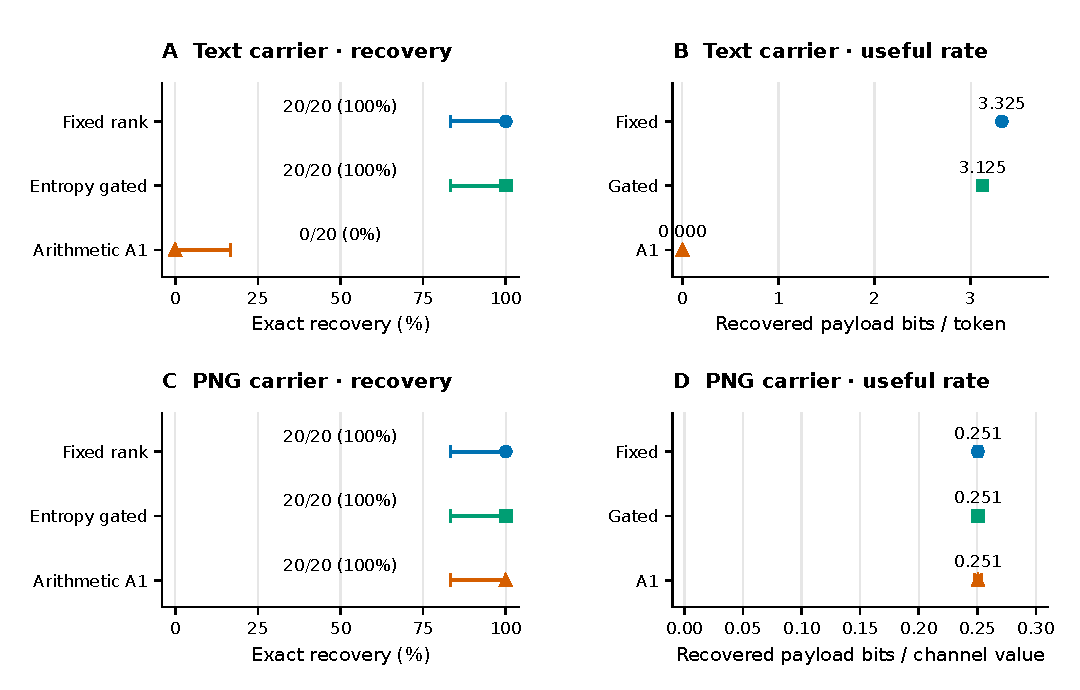
\includegraphics[width=\textwidth]{figures/figure2_recovery_rate.pdf}
\caption{Held-out recovery and exact useful rate for 20 payload groups per direction. Recovery whiskers are the accepted 95\% Clopper--Pearson bounds. Rate whiskers are the accepted stratified group-bootstrap intervals, keeping paired methods together. All failed A1 text transmissions contribute zero goodput. Text and PNG rate axes use different carrier symbols. Zero-width observed rate intervals do not imply universal reliability.}
\label{fig:recovery}
\end{figure*}

Fixed and gated coding recover 20/20 payloads in each direction. Fixed text uses 584 packet positions and 32 completion tokens, giving 3.32468 useful bits/token. Gating adds a mean 39.8 skips, reducing goodput by 0.2000 bits/token [0.1805, 0.2192] and increasing charged pair time by 23.96 seconds [20.34, 27.58]. Whole-carrier mean surprisal decreases by 0.3912 bits/token [0.3079, 0.4764].

All PNG methods recover 20/20, giving mean exact goodput of 0.25054 bits/channel [0.24731, 0.25349], or 0.75161 bits/pixel. Equal rates follow partly from the fixed full canvas and do not imply equal coder capacity. Fixed uses 584 packet channels, gating adds a mean 100.5 skips, and A1's mean packet span is 597.85 channels, including 89.65 zero-bit positions. Ordinary completion fills the remaining channels.

Framing/encryption adds 36 bytes. Texts leave a mean 162.8 padding bytes. Images fill the slot. Including completion, packet transport is 3.79221 bits/token for fixed text, mean 3.56404 for gated text, and 0.78495 bits/channel for every PNG method. A1 text has no complete-packet rate. Its PNG termination position is already included in the packet span, not an extra position.

\subsection{Arithmetic Text Reaches the Capacity Boundary}
All 20 A1 text streams reach the 2,048-token cap before producing the 2,336-bit packet. They recover between 581 and 2,216 packet-prefix bits, with mean 1,456.85. None reaches zero-extension or finite-message termination. Accordingly, none authenticates or delivers useful source bytes, despite the availability of partial information. Mean charged encode-plus-decode time is 826.57 seconds, over six times fixed text, and all that cost remains in the results.

Independent interval, partition and sender/receiver prefix checks agree with all 40 prospective arithmetic audits. Every arithmetic PNG terminates and recovers. Two failed texts have one and three isolated unchanged steps, with longest consecutive run one. A successful PNG also has one. These do not support sustained stagnation as the text-failure cause. Zero-bit steps can continue narrowing an interval without emitting a leading bit.

Cumulative surprisal closely tracks recovered text-prefix information, supporting low information under the cap rather than decoder disagreement or an unexecuted flush. This observed limit is distinct from A1's separately demonstrated stagnation case.

\subsection{Detectability with the Correct Context}
\label{sec:detection-results}


Correct-context scores show that exact recovery and low detectability are different endpoints. Both fixed and gated text have empirical mean-surprisal AUC 1.000, with bootstrap interval [1.000, 1.000]. Every observed stego score exceeds the corresponding ordinary sample range. This is complete empirical separation under the tested observer, not an assurance of perfect future detection. Failed A1 text gives AUC 0.380 [0.260, 0.503]. The below-chance orientation is retained rather than reversed to improve a detector result.

PNG scores are less separated. Fixed mean-surprisal AUC is 0.8850 [0.7425, 0.9850], gating 0.8300 [0.7000, 0.9375], and A1 0.5575 [0.3750, 0.7426]. Arithmetic PNG combines exact delivery with lower observed separation for this score, although its interval spans a wide range around chance. Every cell has 20 scorable stego artifacts and 20 unique matched controls, without exclusions. The secondary log-rank AUCs are 1.000, 1.000 and 0.360 [0.2425, 0.4801] for fixed, gated and A1 text, respectively. PNG values are 0.8400 [0.6825, 0.9650], 0.7700 [0.6299, 0.8975] and 0.5750 [0.4050, 0.7576].

\subsection{PNG Detection Depends on the Tested Context}
\begin{figure*}[t]
\centering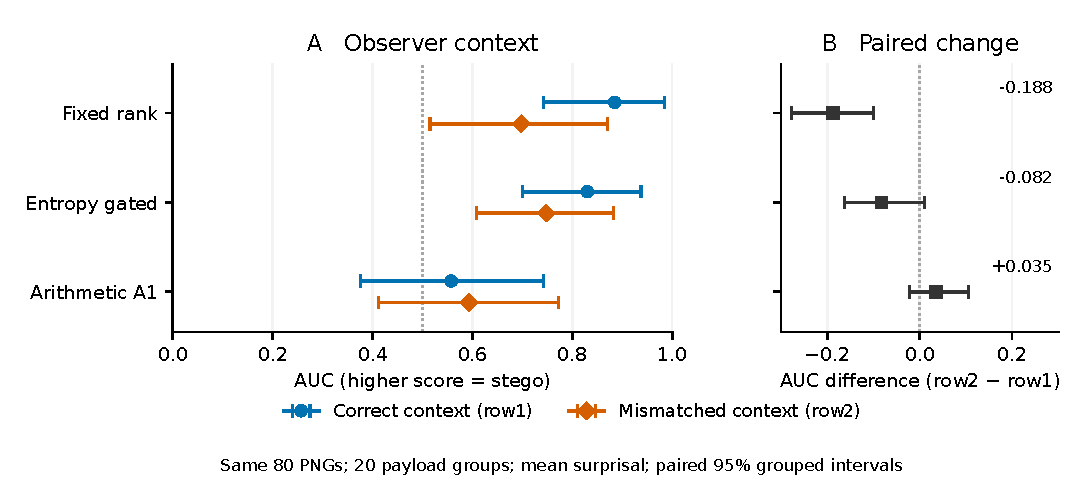
\includegraphics[width=\textwidth]{figures/context_auc.pdf}
\caption{Primary PNG detection with correct row1 and mismatched row2. The same 60 stego PNGs and 20 shared ordinary controls appear in both conditions. Panel B gives paired AUC change, row2 minus row1. Whiskers use the accepted 2,000 length-stratified group draws, jointly retaining observer conditions, methods and control ownership. The observer still knows the exact model and procedure. Row2 is the previously frozen random-RGB row, not a row selected for low detection. Reference lines are not fitted classification thresholds.}
\label{fig:png-context-auc}
\end{figure*}

All 80 retained PNGs are fully scorable under row2. Fixed-rank primary AUC decreases from 0.8850 to 0.6975, a paired change of $-0.1875$ with interval $[-0.2775,-0.1000]$ (Figure~\ref{fig:png-context-auc}). Gating changes from 0.8300 to 0.7475, or $-0.0825$ [$-0.1625$, 0.0100]. A1 changes from 0.5575 to 0.5925, or $+0.0350$ [$-0.0225$, 0.1050]. The fixed reduction is resolved by its paired interval. The gated and A1 changes remain uncertain.

Under mismatch, the primary fixed interval [0.5150, 0.8700] only narrowly excludes 0.5, and its secondary rank-score AUC is 0.6625 [0.4725, 0.8475]. The primary gated interval [0.6074, 0.8825] remains above chance. Thus this mismatch weakens the tested fixed score without removing all information from mean-surprisal detection. A resolved change for one method and an uncertain change for another do not themselves establish different method sensitivities.

Mean row2-minus-row1 score changes are 0.610 bits/channel for controls, 0.334 for fixed, 0.513 for gated and 0.629 for A1. These descriptive shifts narrow the paired fixed-minus-control gap from 0.508 to 0.231. Larger control increases are consistent with, but do not explain, the AUC change. Row1 comes from a generated image and row2 from random RGB values, so context correctness is not isolated from row statistics.

\subsection{Exact GPU Replay Improves Useful Throughput}
CUDA graph replay reduces mean fixed-rank charged encoding from 88.95 to 17.36 seconds and decoding from 88.87 to 17.28 seconds. Combined latency falls from 177.8186 to 34.6417 seconds, a matched 5.133-fold improvement. Pooled useful throughput rises from 0.4799 to 2.4633 recovered bytes per second. These nine fixed timing comparisons include both fresh processes. Gated and A1 single-payload combined times change from 180.25 to 34.61 and 182.85 to 35.11 seconds.

All 11 reference/graph comparisons preserve exact eligible identifiers, rank ordering and float64 probability streams at all 2,976 channels. All 22 PNGs recover identical source bytes, without numerical tolerance or packet rerolls. Graph replay therefore remains an explicit optional mode on this stack. It does not retroactively alter prospective timings. Peak allocated memory is 484.479 versus 473.849 MiB, reserved memory 516 versus 744 MiB and sampled process memory 912 versus 1,176 MiB for reference versus graph. These measures overlap and are not additive. PID-matched GPU activity samples are intermittent, not a sustained-utilization estimate.
